\documentclass[a4paper,12pt]{book}


\usepackage[english]{babel}
\usepackage{blindtext}
\usepackage{microtype}
\usepackage{graphicx}
\usepackage{wrapfig}
\usepackage{enumitem}

\usepackage{amsmath}
\usepackage{index}
\makeindex




\begin{document}

    \title{\Large{\textbf{LaTex Tutorial}}}
    \author{by Esteban}
    \date{December 21}
    \maketitle

    \let\cleardoublepage\clearpage

    \tableofcontents
    \pagenumbering{roman}
    \setcounter{page}{2}
   

    \chapter{Chapter Name}
    \blindmathtrue
    \blindtext[3]
    \enlargethispage{\baselineskip}

    \section { A section}
    \blindtext[2]
    \enlargethispage{\baselineskip}
    \blinditemize
    \blindenumerate
    \blinddescription

    \section*{Spacing}
    \LaTeX\
    just random\\
    the second line is indented. if  wwe  use spaces \\[10pt]
    \% \$ \$ \_ \textbackslash


    \section[List]{Lists Recipe }
    
    \begin{itemize}
        \item  cup 1
        \item  cup 2
        \item  cup 3
        \begin{itemize}
            \item 1 table textbackslash
            \item 1 tbs lsa
            \item example of list in list
        \end{itemize}
        \item cup 6
    \end{itemize}
\setlist{nolistsep}

    \section {Smoothie}
    \blindtext[2]
    \enlargethispage{\baselineskip}
 

\newpage
    \section {Pefect Meal Recipe}
    \begin{enumerate}[label= \arabic*,font=\bfseries]
        \item Add the following and cook
        \begin{itemize}
            \item toast
            \item milk
        \end{itemize}
        \item end
    \end{enumerate}
    \bigskip

    \begin{description}
        \item[Philtrum] And descriptions here
    \end{description}

    \begin{tabbing}
        Customer\=Name \hspace*{1.5 cm}\= Street \hspace*{1.5cm} \= City \\
        \>name here \> quito \> conocoto \\
    \end{tabbing}


\begin{table}
    \begin{tabular}{c|c|c}
        \textbf{Name}&\textbf{command}&\textbf{sample text}\\
        \hline
        emphasize&\verb|\emph| & \emph{abcd}\\
        
    \end{tabular}
    \caption{ways to emphasize text} \label{sec:typeemp}
\end{table}

\begin{tabular}{@{}*3l@{}}
    \multicolumn{2}{c}{name} &
    \multicolumn{1}{c}{age}\\
    first & Last & \\
    \hline
    eset & bananas & 44\\
    sally & smith & 42 \\
    
\end{tabular}\\

\pagebreak
    \section {use image 1}
    \begin{figure}[ht]
        \centering
        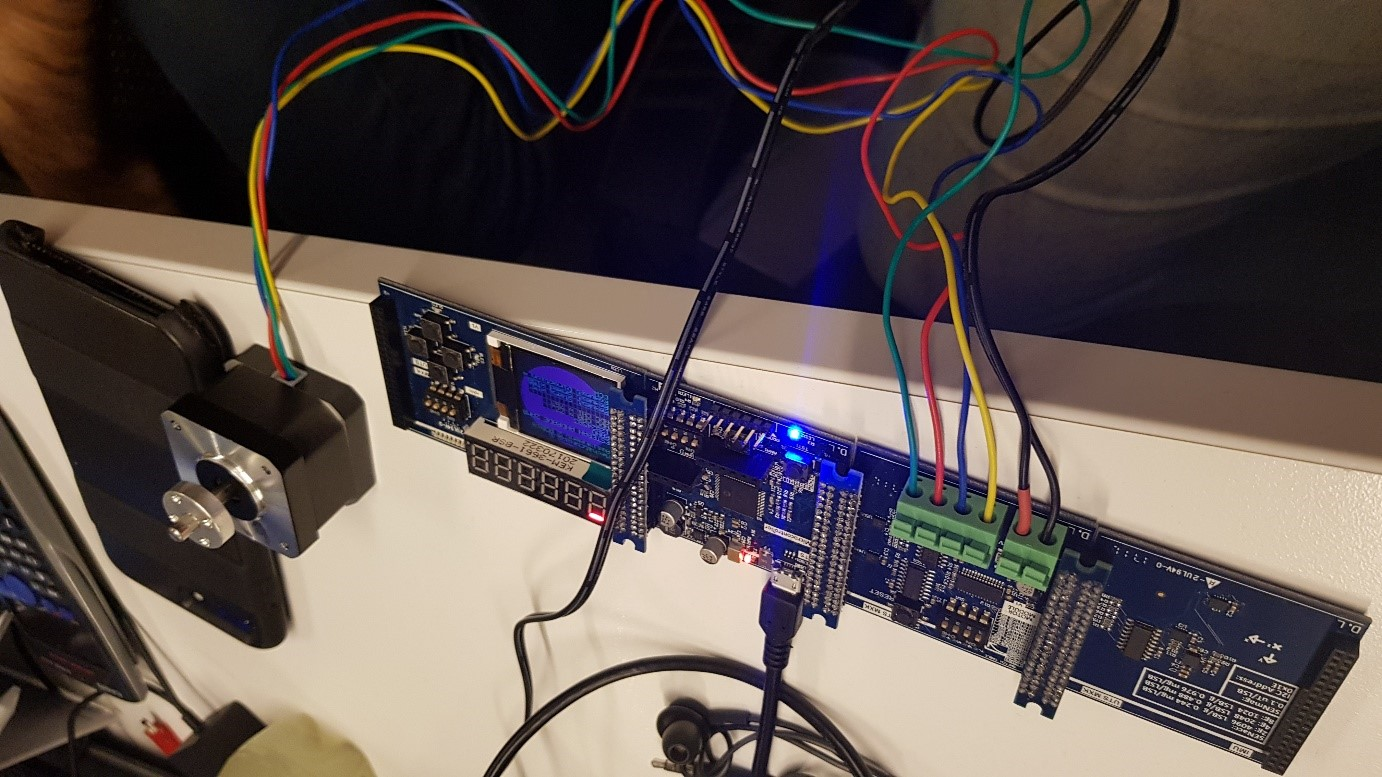
\includegraphics[width=8cm]{microcontoller.jpg}
    \end{figure}
    \blindtext[9]



\newpage
    \section*{wrap image}
    \begingroup
    \setlength{\intextsep}{0pt}
    \setlength{\columnsep}{15pt}

    \begin{wrapfigure}{r}{0.45\textwidth}
        \centering
        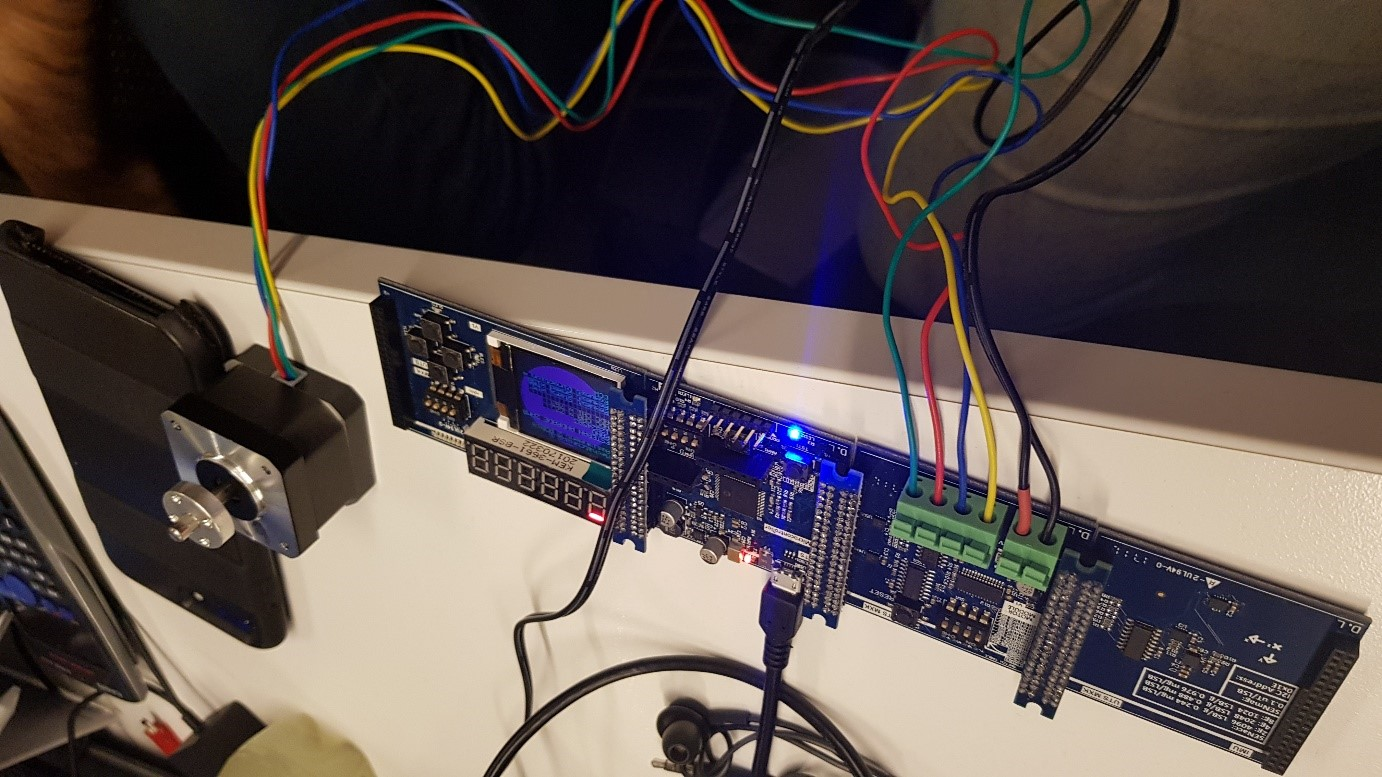
\includegraphics[width=\linewidth]{microcontoller.jpg}
        \caption{pretty picture}\label{fig:prettypic}
    \end{wrapfigure}
    \blindtext[1]
    
    \endgroup

\section[Type]{\textsf{Type emphasus \& Sizing}} 
\label{sec:typeemp}
\itshape italic


\section{Math formulas}
\begin{flalign*}
    &ax^2+bx+c=0 &\\
\end{flalign*}

\begin{align}
    &ax^2+bx+c=0 &\\
\end{align}

this \(ax^2+bx+c=0\) is the quadratic eq \\

$x=\frac{-b\pm\sqrt{b^2-4ac}}{2s} $\\

vectors $\vec{a}\cdot\hat{x}=a_x $\\
$\begin{pmatrix}
    1&2\\
    3&4 
\end{pmatrix}$


\section{text columns}
{
    \centering
    get in the middle of me \\
    oka \\[10pt]
}
\quad\parbox{4cm}{i used to think that this was lol}
\quad\parbox{2cm}{i used to think\-that\-this was lol}
\quad\parbox{2cm}{\raggedright i used to think that this was lol}
\quad\parbox{2cm}{\raggedleft i used to think that this was lol}\\

\begin{minipage}{5 cm}
   One aasdffffffffffffffffffffffffffffffffffffffffffffffffff 
\end{minipage}

\section{Referencing}
the answer to this is not.
\footnote[2]{author unkown}\\[5pt]

there is a great table thingy~\ref{sec:typeemp} on page ~\pageref{sec:typeemp}

how i learn my ABDS \cite{ABCAFB}.

\begin{thebibliography}{books}
    \bibitem{ABCAFR} Walter abish \emph{The alphabetical Africa},174
\end{thebibliography}

index test when i baas kajshshah - {\index{Rodney}rodnet and}\\{2pt}

\blindtext

\clearpage
\addcontentsline{toc}{chapter}{index}
\printindex

\end{document}